\chapter{Software architecture}

% TODO: En este apartado empiezo a poner diagramas, los pongo a color o
% mejor en blanco y engro??

“Most systems work better they are kept simple rather than complicated”
\cite{kiss-wiki}. This is the main statement of the KISS principle, acronym for
“Keep it simple, stupid”. KISS philosophy is very used on software development
because code tends to chaos. If the implementation of a functionality is not
properly thought, it adds complexity to the program work flow. Therefore, to
reduce the architecture entropy is one of the main design patterns.

Model-View-Controller (MVC) is a well-known software architecture that consists
on the use of this tree elements to build a user interface. It was introduced 
by Trygve Reenskaug in the seventies \cite{mvc-past-present}. When web
applications appeared, this model was applied in many important projects
like \href{https://support.microsoft.com}{Microsoft Support}. 

% TODO: NO SE COMO PONER UNA WEB COMO EJEMPLO

\begin{figure}[htb]
	\begin{center}
		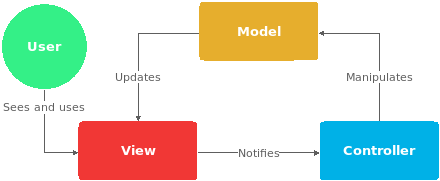
\includegraphics[width=0.5\textwidth]{./figures/mvc.png}
		\caption{Diagram of interactions within the MVC pattern.
				 \cite{mvc-wiki}}
		\label{F:mvc}
	\end{center}
\end{figure}

As shown on Figure \ref{F:mvc}, it is a simple model to represent
a user interface (UI). The UI visual representation is managed by the view.
Each time the user performs an action, view notifies controller and it modifies
the current model. Since view is watching it, the change is detected and view
is affected.

The problem is that this architecture becomes complex and complex while 
increasing the number of view. Actions from a view can affect other views'
model and this changes can trigger other actions. This complexity could even
generate unexpected loops as Figure \ref{F:mvc-complex} proves.


\begin{figure}[htb]
	\begin{center}
		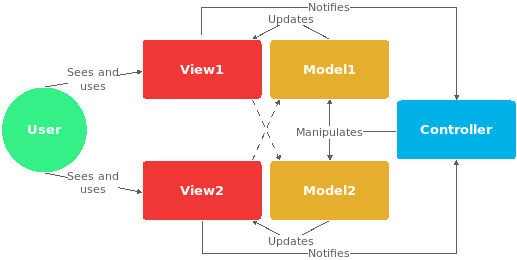
\includegraphics[width=0.6\textwidth]{./figures/mvc-complex.png}
		\caption{Diagram of interactions within the MVC pattern with many views}
		\label{F:mvc-complex}
	\end{center}
\end{figure}

\section{Flux-like architecture: React + Redux}

In order solve the MVC scalability problem, Facebook proposed Flux
\cite{flux-web}. Flux is the application architecture that Facebook uses for
building client-side web applications. To solve the loop problem, they devise
an “unidirectional data flow with changes described as plain objects”.

\begin{figure}[htb]
	\begin{center}
		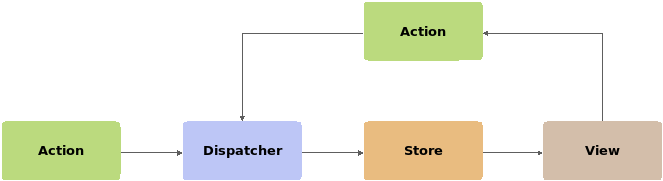
\includegraphics[width=0.7\textwidth]{./figures/flux.png}
		\caption{Diagram of Flux}
		\label{F:flux}
	\end{center}
\end{figure}

Even through Figure \ref{F:flux} appears to have a loop, with Flux things are
much easy to handle. View just wait change events produced by the store and
render themselves using the current state information. Note that render
processes do not need to call any action.

\subsection{React}

React is an implementation of Flux view piece. It is a component-based 
JavaScript library to build user interfaces \cite{react-web}. Each React
component can have input properties and a state, and must implement a render
function. Furthermore, to make things easier, React supports JSX which are
JavaScript files where HTML code can be used.


\begin{codefigure}{React hello world}{F:react-hello-world}
	\jsxexternal[
		classoffset=1,
		morekeywords={HelloMessage, React, Component, ReactDOM},
		classoffset=2,
		morekeywords={<HelloMessage},
	]{source/react-hello-world.jsx}
\end{codefigure}

Figure \ref{F:react-hello-world} shows up an example of React component. It has
a no state, a property call name and an easy render function to create a div.
Render functions can also have components inside themselves. That way, React
creates a component tree \ref{F:react-tree}.

\begin{figure}[htb]
	\begin{center}
		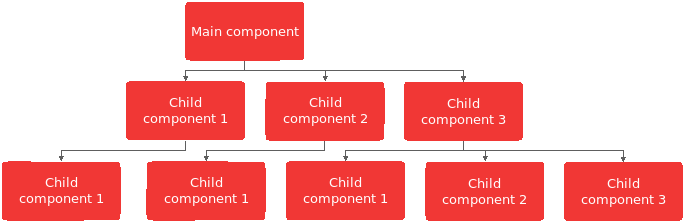
\includegraphics[width=0.7\textwidth]{./figures/react-tree.png}
		\caption{React tree}
		\label{F:react-tree}
	\end{center}
\end{figure}

Components may need to perform actions. Those cannot be performed on render 
function, as seen before. To do that, each component have a lifecyle. It 
consists of a functions' set that are called when some external actions happen. 
Most used ones are \textit{"componentWillMount"} and 
\textit{"componentWillUnmount"}. Components also can listen to its view
elements to perform actions.

\subsection{Redux}

Redux was inspired by several important qualities of Flux. Like Flux, Redux
prescribes that you concentrate your model update logic in a certain layer of
your application (“stores” in Flux, “reducers” in Redux) \cite{redux-prior-art}.

The model is called state and it is contained inside a store. Actions are
dispatched using the store. Then, those actions can modify the state using
reducers.

But to exploit the full potential of Redux, tree principles must be followed
\cite{redux-principles}.

\begin{description}
	\item [Single source of truth]
	The state can be stored easily if just one store is used. Furthermore, the
	application will be easy to debug.
	
	\item [State is read-only]
	The only way to modify the state is using actions. Each time the state
	changes, a new state must be created.

	\item [Changes are made with pure functions]
	Reducers must be pure functions, that means, using the same initial state,
	repeating the same list of actions must produce the same final state.

\end{description}

\subsubsection{Action creators}

An action is a plain JavaScript object that contains a field called type to 
identify it and other optional fields that are the payload. Same type of action
can be created in many places of the code so it is extremely recommended to use
action creators.

Action creators are functions that create those objects. Normally are defined
using lambdas. An example of action creator is shown on Figure
\ref{F:redux-action-creator}.

\begin{codefigure}{Redux action creator}{F:redux-action-creator}
	\jsexternal{source/redux-action-creator.js}
\end{codefigure}

\subsubsection{Reducers}

Reducers aim to return new states each time an action is produced. They must be
implemented using pure functions. Tree statements must be followed:

\begin{description}
	\item [Mapping]
	Same input always returns the same output.\\
		\textbf{KO}: \jsinline{ const mult = (x) => Math.random() * x; }\\
		\textbf{OK}: \jsinline{ const mult = (x) => 2 * x; }

	\item [Avoid side effects]
	Cannot produce changes outside. \\
		\textbf{KO}: \jsinline{ const title = (x) => document.title = x; }\\

	\item [No external mutable]
	Output won't change due to any implicit action.\\
		\textbf{KO}: \jsinline{ const rename = (obj, val) => obj.name = val; }\\
		\textbf{OK}: \jsinline{
			const rename = (obj, val) => \{ ...obj, name: val \}; 
		} \\
\end{description}

Figure \ref{F:redux-reducer} shows up an example of reducer for action shown on
Figure \ref{F:redux-action-creator}

\begin{codefigure}{Redux reducer}{F:redux-reducer}
	\jsexternal{source/redux-reducer.js}
\end{codefigure}



\subsubsection{Selectors}

\subsection{Complements}

\subsubsection{Redux Observables}

\subsubsection{React Redux Form}

\subsubsection{React Tables}

\section{The Sleuth Kit JavaScript}

